%
% Another appendix chapter
\chapter{Toward Application: Walking}\label{chap:walking}
The control strategy for a static, standing case presented in the previous chapter is two-dimensional. If the robot is walking, the motion of the \ac{CoM} relative to the ground reference point might not be \textit{aligned} with the direction of the error, as the horizontal \ac{CoM} position can lie outside the support polygon. In this chapter, the bang-bang control law of Chapter \ref{chap:standing} is extended for the use in \ac{3D}.
% Experimental Setup
\section{Experimental Setup}
With the same motivation as in the previous chapter of applying a maximum acceleration possible in a worst-case scenario, a bang-bang control law can be used. In this section, to determine \textit{when} to turn the bang-bang controller on in \ac{3D},  tests are conducted preliminary to developing a controller. 

In the tests, a push is applied in the beginning of the \ac{SS} while the robot is walking. The stepping parameters used for the test situation are given in Table \ref{tab:stepping}, which are the default stepping parameters during testing in simulation. In \figref{fig:valwalkingtest}, the test setup in simulation is shown. The limited foothold options display that footstep location adjustment is not available as a balance strategy. In \figref{fig:3foot}, the \ac{ICP} and \ac{CMP} reference trajectory and the measured \ac{CoM} trajectory, without application of a push are made visible. 
\begin{table}[ht]
\caption{Stepping Parameters} % title of Table
\centering % used for centering table
\begin{tabular}{c c c } % centered columns (4 columns)
\hline\hline %inserts double horizontal lines
Parameter & Value & Unit \\
%heading
\hline % inserts single horizontal line
Step Legth & 0.5 &  [m]\\
Step Width & 0.25 & [m]\\
\acs{SS} Time & 0.6 & [s]\\
\acs{DS} Time & 0.15 & [s]\\
%[1ex] % [1ex] adds vertical space
\hline %inserts single line
\end{tabular}
\label{tab:stepping} % is used to refer this table in the text
\end{table}
\begin{figure}[h]
\centering
  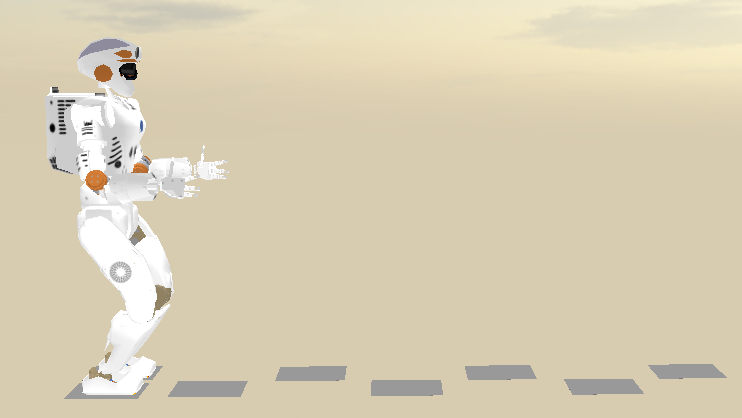
\includegraphics[width=.8\linewidth]{STYLESTUFF/valwalkingtest.png}
   \caption{Test setup for push recovery during walking in simulation. The limited foothold options show that footstep adjustment is not available as a balance strategy.}
    \label{fig:valwalkingtest}
\end{figure}
\begin{figure}[h]
\centering
  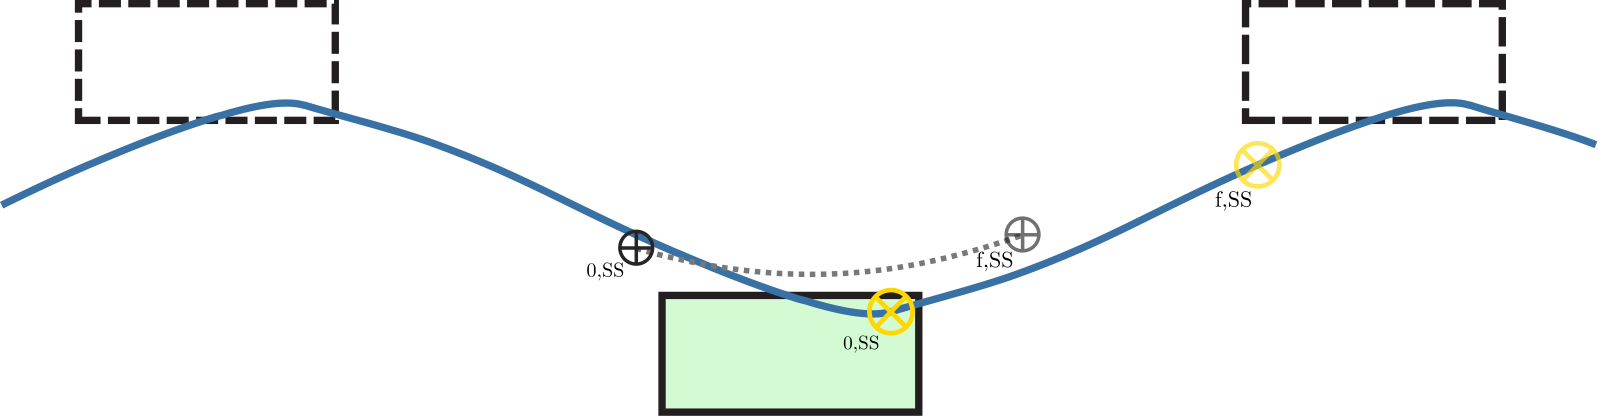
\includegraphics[width=.8\linewidth]{STYLESTUFF/ICPplan3StepComICPrSS.png}
   \caption{Trajectories during \ac{SS} in the horizontal plane (gray dotted lines). The gray area is the current footstep position.}
    \label{fig:3foot}
\end{figure}
%Preliminary observations

The following properties are observed, when applying pushes in different direction in the start of \ac{SS}:
\begin{enumerate}
	\item The direction of the \ac{ICP} error stays often approximately the same until transition to \ac{DS}.
	\item If the \ac{ICP} error is directed in the sagittal plane, the desired \ac{CMP} often remains somewhat in the same location.
	\item If the \ac{ICP} error is directed  in the coronal plane, the desired \ac{CMP} slides from back to the forth of the foot.
	\item The configuration and velocity near transition to \ac{DS} affects the robots ability to put its swing leg down at the desired time. 
\end{enumerate}
These properties are used as assumptions in the development of a control law.
% Methods
\section{Method}

\subsection{Avoiding Generating Angular Momentum Rate}
First, the control law of the previous chapter is made suitable for $\rcmpd$ locations outside the support polygon. The motivation in the development of a control law is to request as less as possible additional angular momentum rate compared to the default setup, when using \ac{CoM} height variations for balance control. Therefore, the vertical motion controller generates and added desired momentum rate on top of the default controller. Under the assumption that the difference in $\rcopd$ and $\rcmpd$ is directly related to the resulting torque about the \ac{CoM}, the following is derived:
\begin{align}
    \dotldxy &= \frac{\cxy-\rcmpd}{z_0}(mg+\dotldz),\\
&=\frac{\mathbf{c}_{xy}-(\rcopd+\frac{\taucom}{(mg+\dotldz})}{z}(mg+\dotldz), \\
&=\frac{\mathbf{c}_{xy}-\rcopd}{z}(mg + \dotldz)- \frac{\taucom}{z},
\end{align}
If the location of $\rcmpd$ is outside the polygon, the vertical motion controller uses $\rcopd$ for additional height variation. The computation reads as follows:
 \begin{align}
\dot{\mathbf{l}}_{xy,d}&=\frac{\mathbf{c}_{xy}-\rcopd}{z}(mg+\dotldz) - \frac{\taucom}{z},\\
&=\underbrace{ \frac{\mathbf{c}_{xy}-\mathbf{r}_{cmp,d}} {z_0}mg}_{\dotldxylip}  + \underbrace{\frac{\mathbf{c}_{xy}-\mathbf{r}_{cop,d}}{z}\dotldz}_{\dotldxyheight},
\end{align}
where $\dotldxyheight$ is the additional desired horizontal linear momentum rate from the vertical motion controller and $\dotldxylip$ the momentum rate from the default control law.

In Figure \ref{fig:rcopdvsrcmpd}, it is visually explained in \ac{2D} how this computation of $\dotldxy$ does not require additional angular momentum from the robot. However, the resulting \ac{CMP} location would be different.

\begin{figure}
\centering
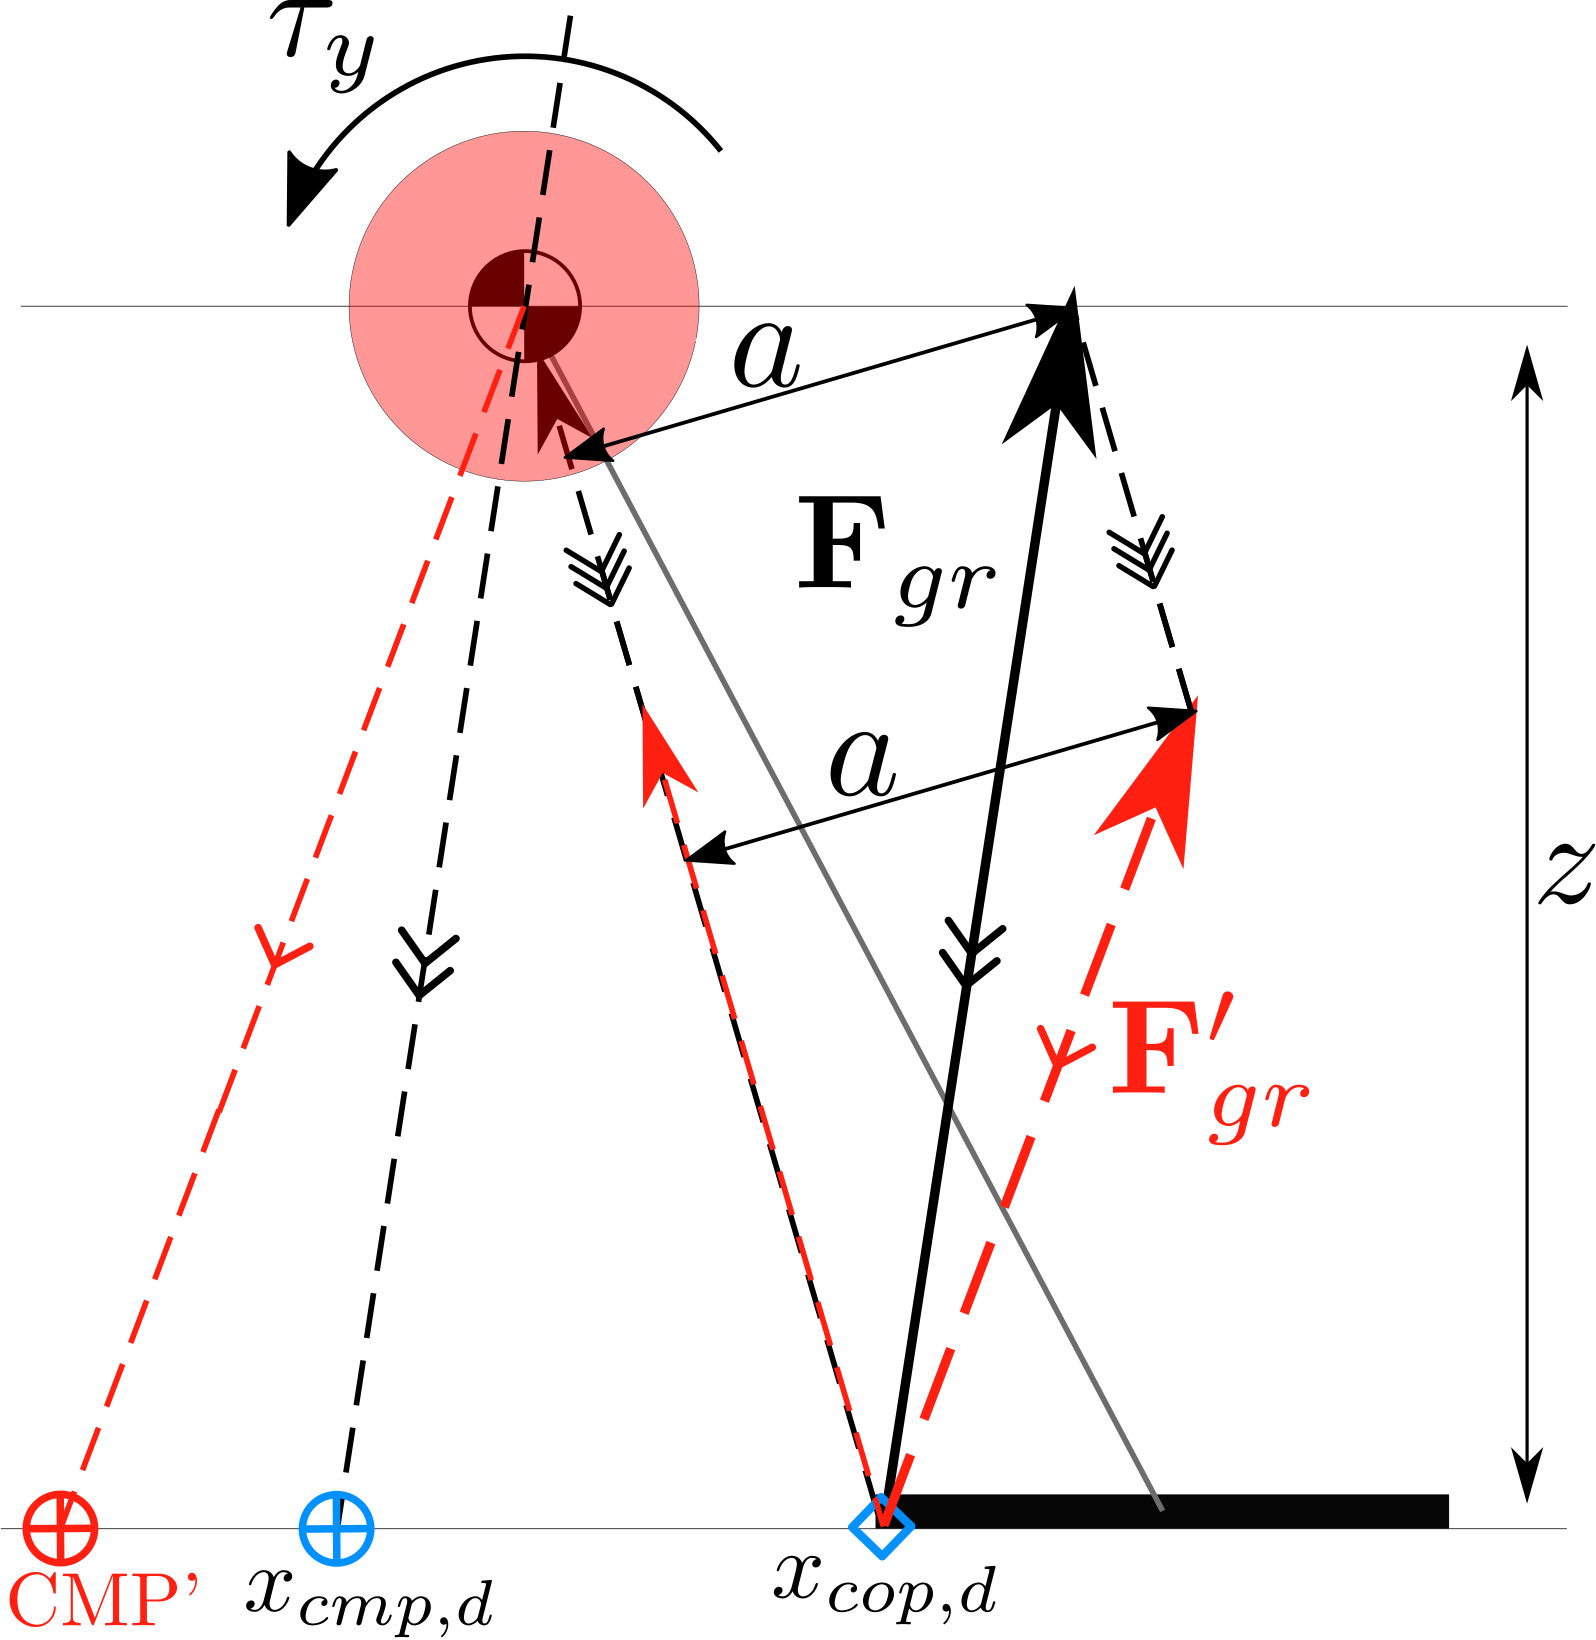
\includegraphics[width=0.45\textwidth]{STYLESTUFF/2DControlStrategyViz.png}
\caption{Requesting additional horizontal momentum rate based on $\rcopd$ will not need additional angular momentum to be achievable, as the scalar offset $a$ is equal. However, the resulting \ac{CMP} will be in a different location than $\rcmpd$.}
\label{fig:rcopdvsrcmpd}
\end{figure}
\subsection{Alignment Angle and Relative Distance}
If the \ac{CoM} is outside the support polygon, the local virtual leg between $\rcopd$ and the horizontal \ac{CoM} location $\cxy$ may not be aligned with direction of the \ac{ICP} error $\icpe$. This results in the leg applying force in a different direction than is needed to cancel the error, which can result in additional error in another direction. Also, if $\cxy$ is close to the polygon edge, the distance with $\rcopd$ might be very small, such that height changes have little to potentially no effect. To take these two aspects into account, the following variables are introduced, which help to determine when to use \ac{CoM} height variation for balance:
\begin{itemize}
	\item $\phi$: the alignment angle between the virtual leg between $\rcopd$ and $\cxy$ and the \ac{ICP} error $\icpe$;
	\item $\delta$: the effective distance between $\rcopd$ and $\cxy$. The is the distance between the two points in the direction of the \ac{ICP} error $\icpe$.
\end{itemize}

In \figref{fig:phiViz}, the two variables are graphically explained using the stance foot position of \figref{fig:3foot}. $\rcmpd$ is allowed to move a small distance outside the polygon. In \figref{fig:phiVizc}, the angle $\phi$ is zero and $\delta$ is relatively large. This is a relatively suitable error for height control. In \figref{fig:phiVizd}, the angle $\phi$ is $90$ degrees and therefore the distance $\delta$ is zero. In this configuration, \ac{CoM} height variation would not help driving the error back. Furthermore, an additional error would occur orthogonal to the current $\icpe$.
\begin{figure}[h]
\centering
  \begin{subfigure}{0.49\textwidth}
    \centering
  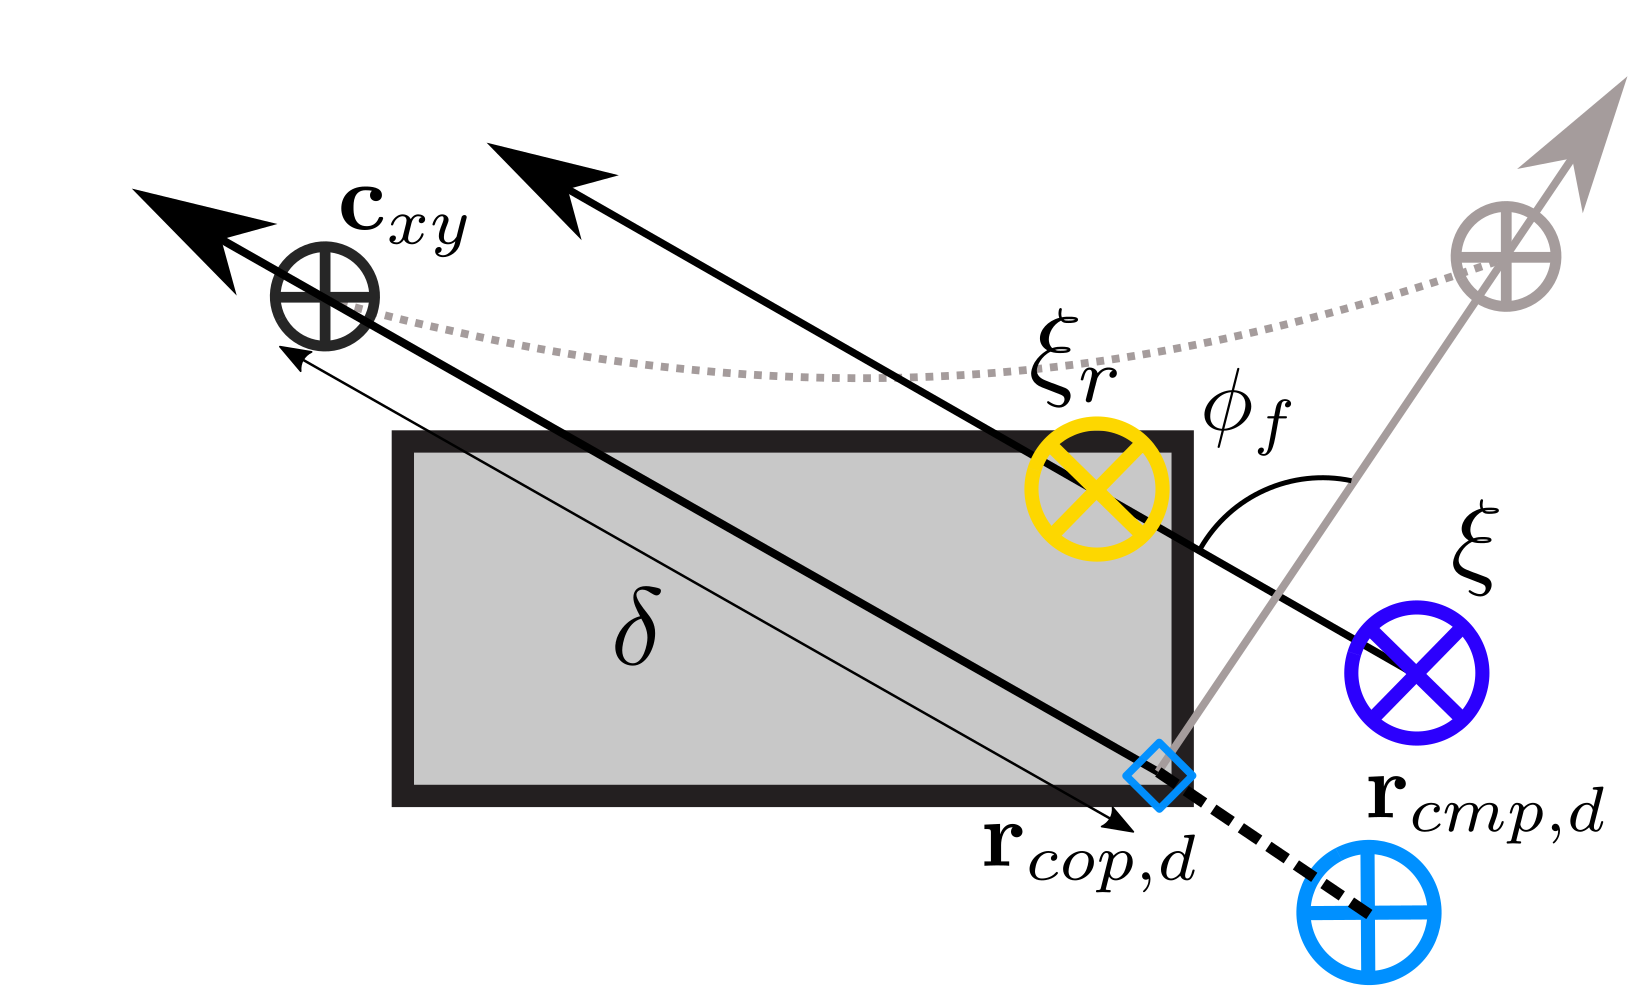
\includegraphics[width=.7\linewidth]{STYLESTUFF/ICPplanStartSSPhiViz0.png}
    \caption{}
     \label{fig:phiVizc}
  \end{subfigure}
  \begin{subfigure}{0.49\textwidth}
    \centering
  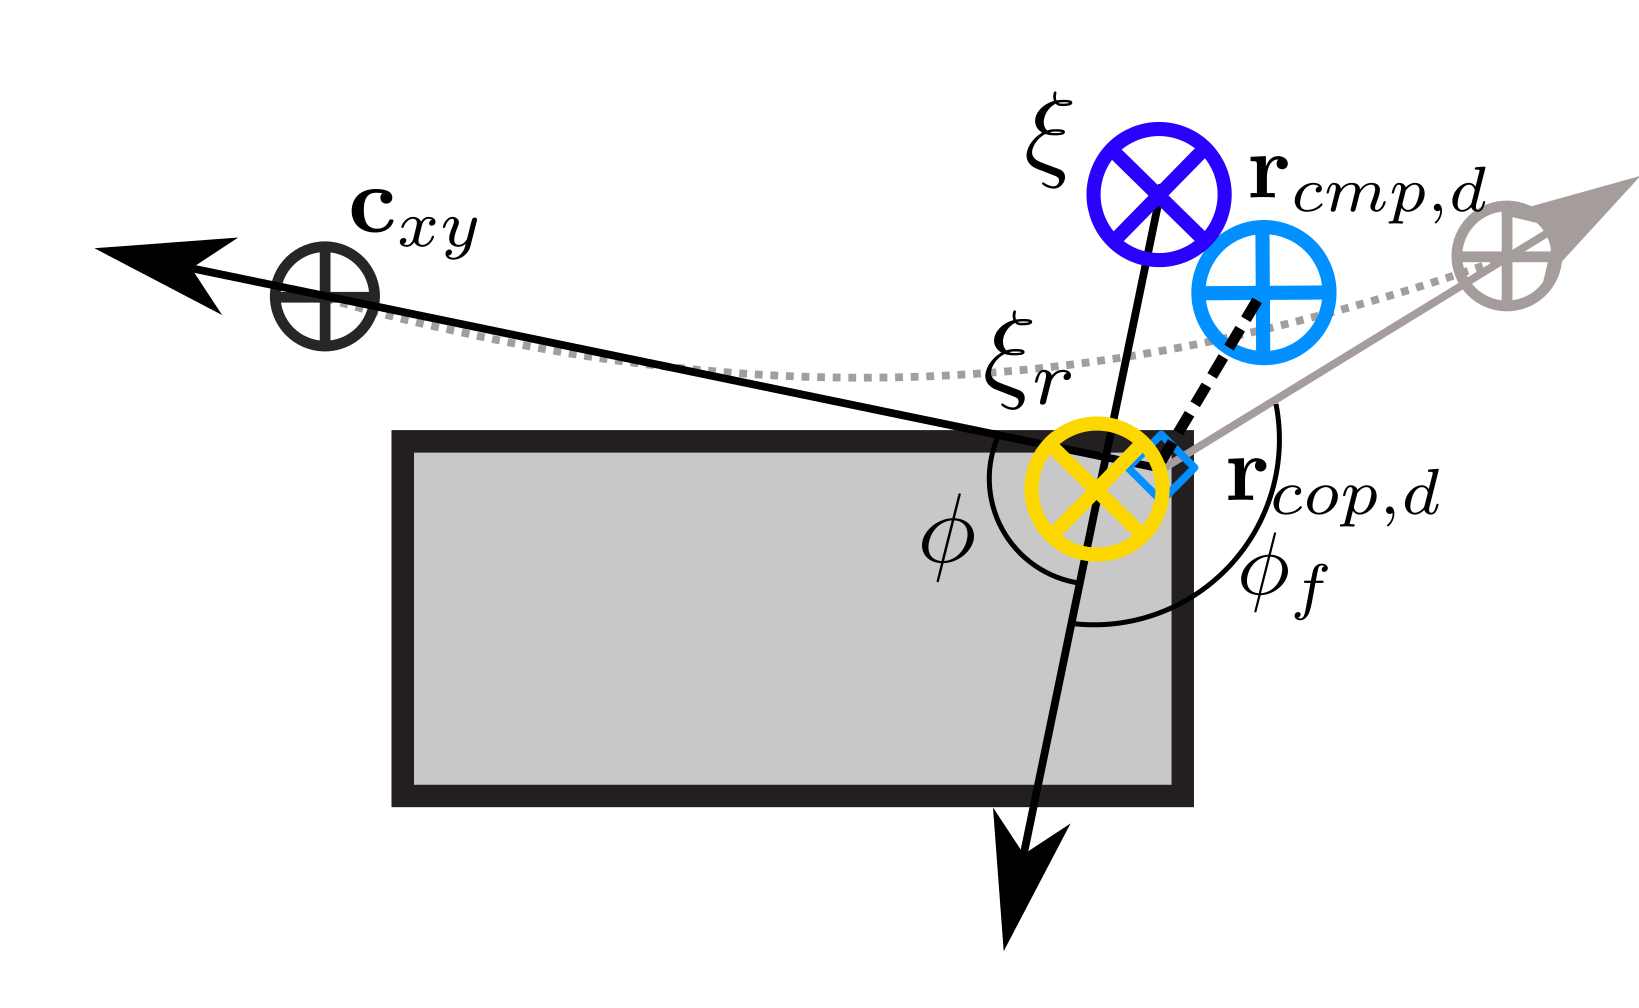
\includegraphics[width=.7\linewidth]{STYLESTUFF/ICPplanStartSSPhiViz90.png}
    \caption{}
     \label{fig:phiVizd}
  \end{subfigure}
  \caption{Vizualizations of $\phi$ and $\delta$ for the configuration at start of \ac{SS}.}
  \label{fig:phiViz}
\end{figure}

\subsection{Actions}
The alignment angle $\phi$ and the relative distance $\delta$ are used to select a control action, if the $\rcmpd$ crosses the polygon edge. From the assumptions of the preliminary observations $1$ and $2$, it is assumed that the angle $\phi$ will be dependent on the current $\icpe$ and $\rcopd$ throughout \ac{SS} if $\icpe$ is directed in the sagittal plane. Therefore, the additional variables $\delta_f$ and $\phi_f$ are used, which are the expected alignment and distance in the end of \ac{SS}, based on the \ac{CoM} location coming from the \ac{ICP} planner. Also, from assumption $3$, $\phi$ is not used if a push is in the coronal plane. Throughout \ac{SS}, the whole foot length is available for future $\rcmpd$ placements that could correct any additional error. Based on the discussed variables, the following three actions can be selected:
\begin{itemize}
	\item \textbf{Positive alignment}: At the current control tick, $\phi$ is relatively misaligned and $\delta$ relatively large for a push in the sagittal plane, or $\delta$ is relatively large for a push in the coronal plane. Also, $\phi$ has to be smaller than $\frac{1}{2}\pi$ [rad], as the virtual leg must be in direction of the \ac{ICP} error to make additional force effective. A bang-bang action is activated that starts with a positive `bang'.
	\item \textbf{Prepare}: At the current control tick, $\phi$ is relatively misaligned or $\delta$ is relatively small, but $\phi_f$ and $\delta_f$ are at values suitable for the positive alignment phase. The \ac{CoM} height is gradually lowered to the minimum height, after which the `bang-bang' action of the positive alignment phase is activated.
	\item \textbf{Default}: All decisions variables $\phi$, $\delta$, $\phi_f$ and $\delta_f$ are at such values, that vertical \ac{CoM} motion does not improve recovery. The default height control law is used and no additional height changes are considered.
\end{itemize}

In \figref{fig:phi}, four cases are shown for different actions. In \figref{fig:phiViza} and , a positive alignment action is introduced, as $\phi$ is relatively small and $\delta$ relatively large. In \figref{fig:phiViza}, the prepare action is used, as $\delta_f$ and $\phi_f$ are more suitable for height control. In \figref{fig:phiVize}, the positive alignment action is used, as the current $\delta$ is relatively large. In \figref{fig:phiVizf}, the default action is activated, as $\delta$ is small throughout \ac{SS}.
\begin{figure}[h]
\centering
  \begin{subfigure}{0.49\textwidth}
  \centering
  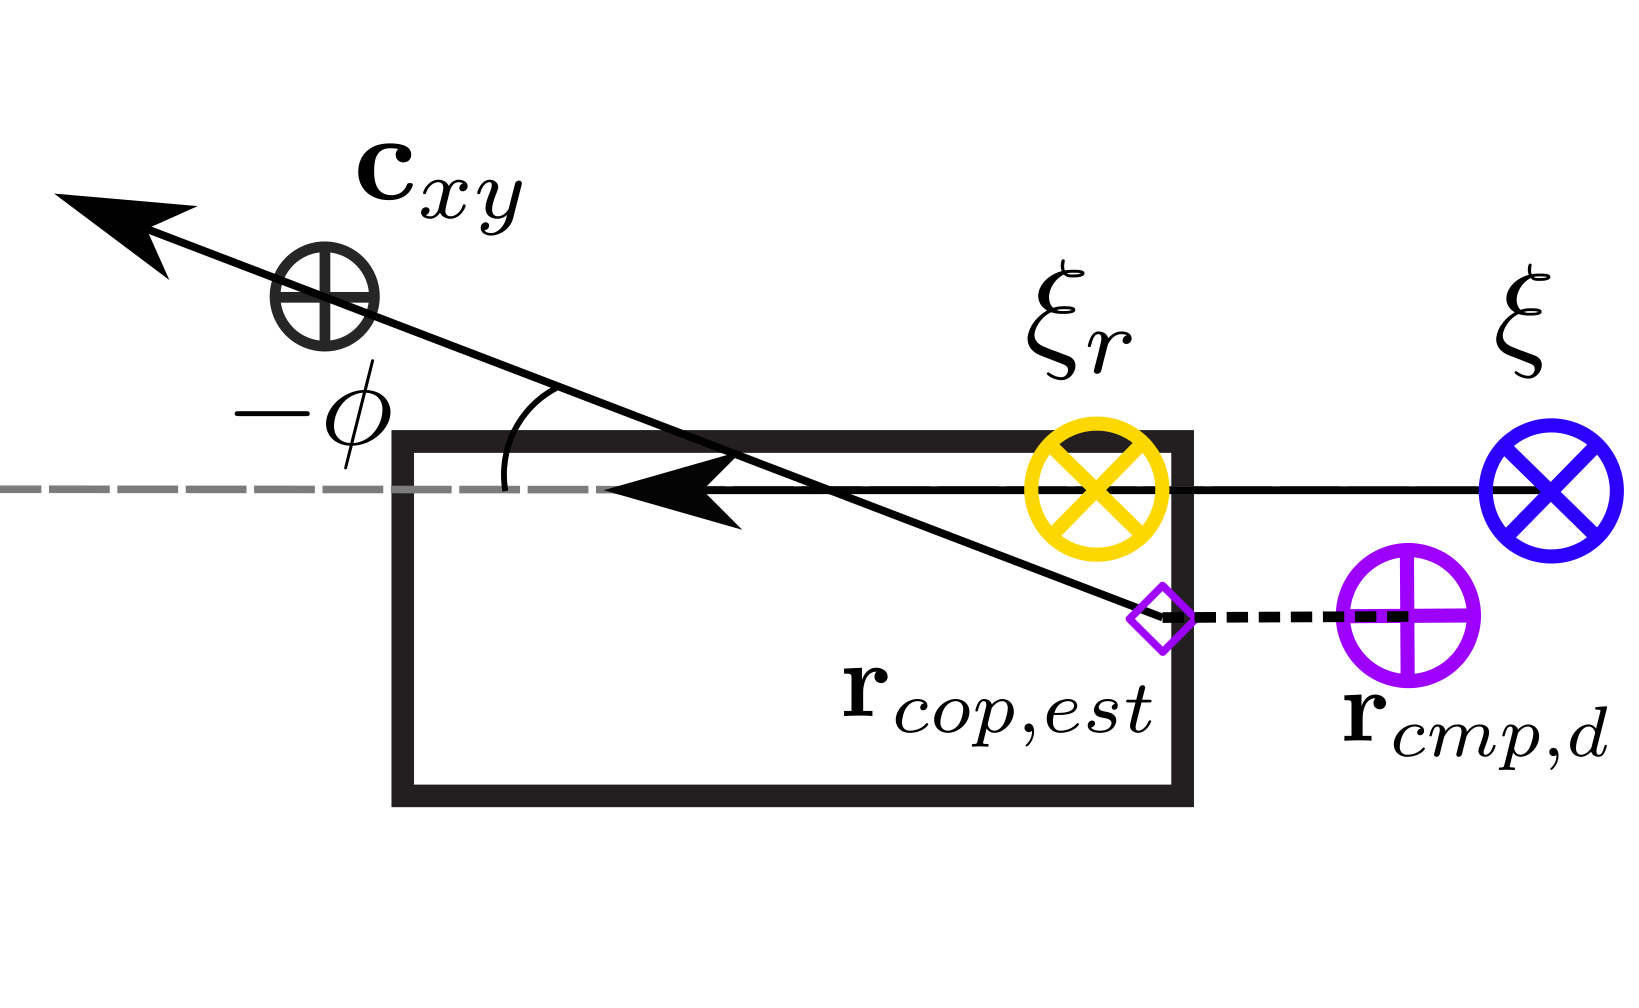
\includegraphics[width=.7\linewidth]{STYLESTUFF/ICPplanStartSSPhiVizNegError.png}
   \caption{}
    \label{fig:phiViza}
  \end{subfigure}
  \begin{subfigure}{0.49\textwidth}
    \centering
  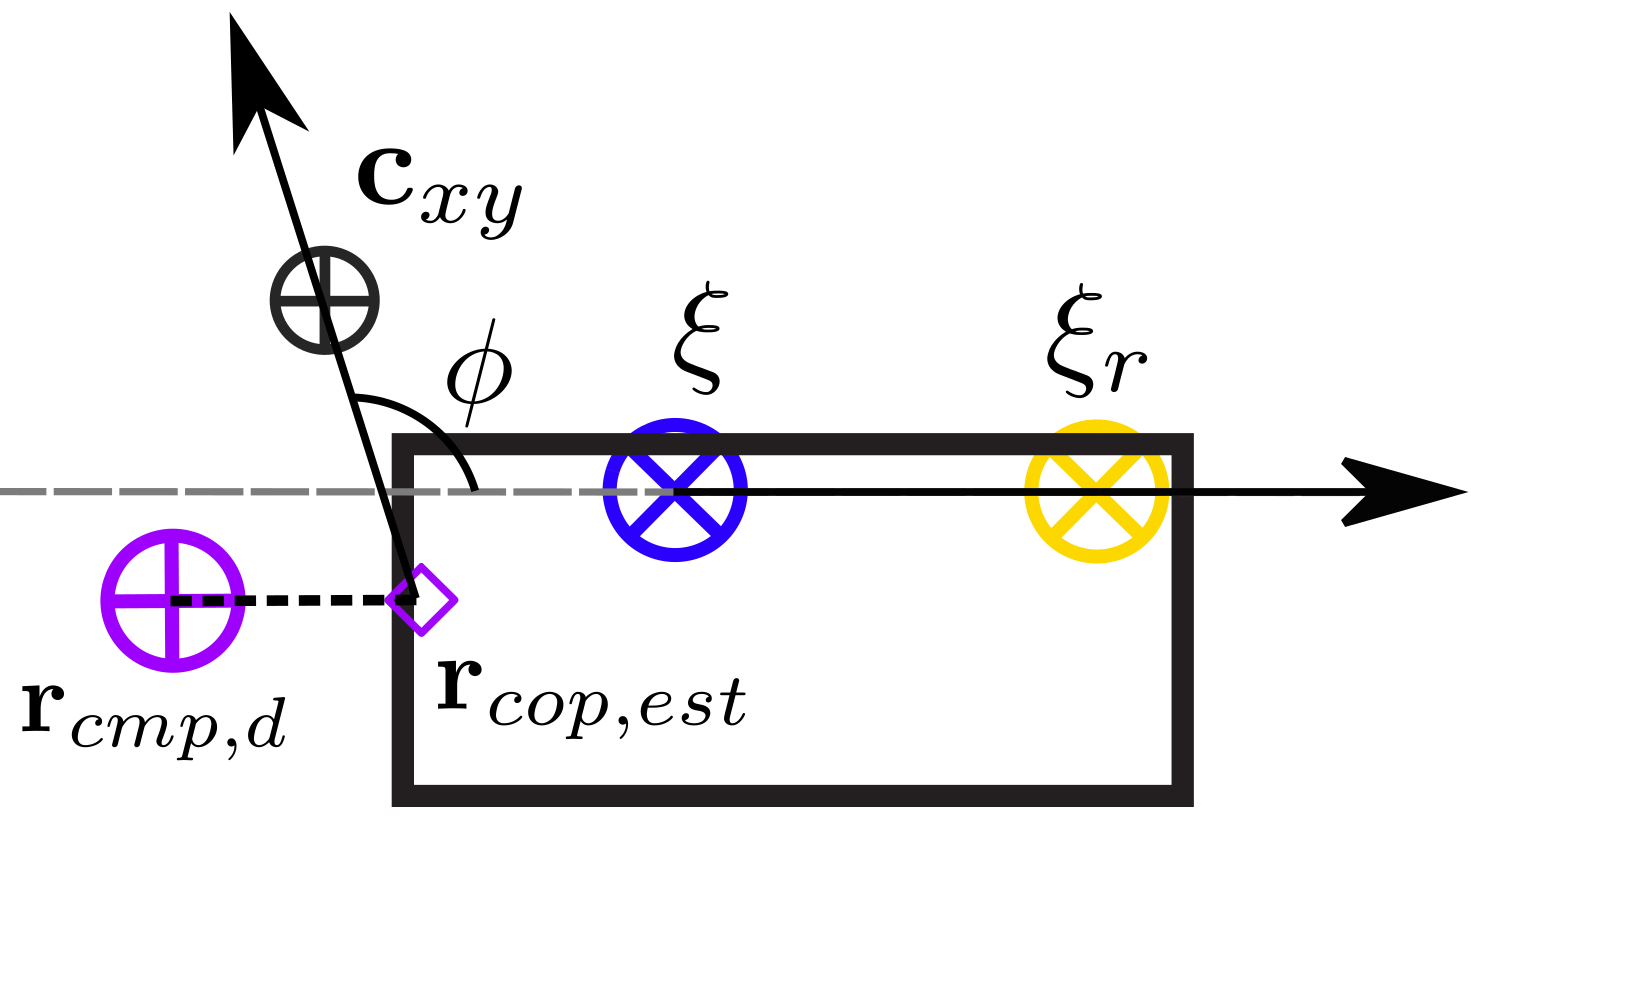
\includegraphics[width=.7\linewidth]{STYLESTUFF/ICPplanStartSSPhiViz.png}
  \caption{}
   \label{fig:phiVizb}
  \end{subfigure}
    \begin{subfigure}{0.49\textwidth}
    \centering
  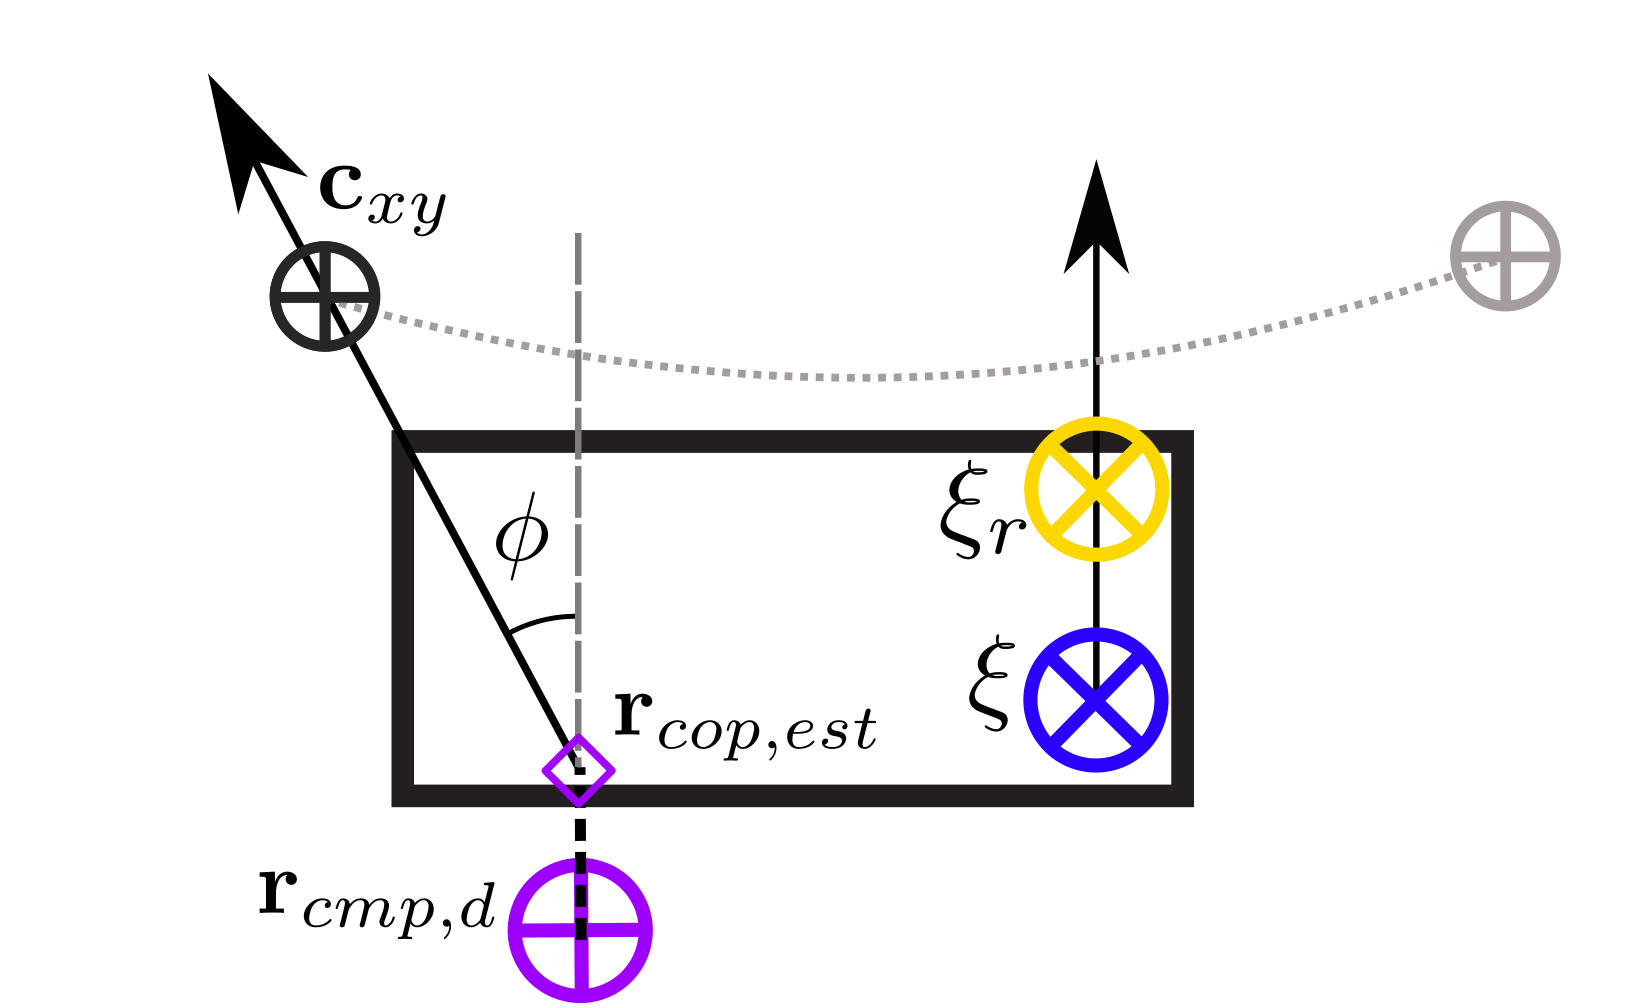
\includegraphics[width=.7\linewidth]{STYLESTUFF/ICPplanStartSSPhiVizLeftError.png}
    \caption{}
     \label{fig:phiVize}
  \end{subfigure}
  \begin{subfigure}{0.49\textwidth}
    \centering
  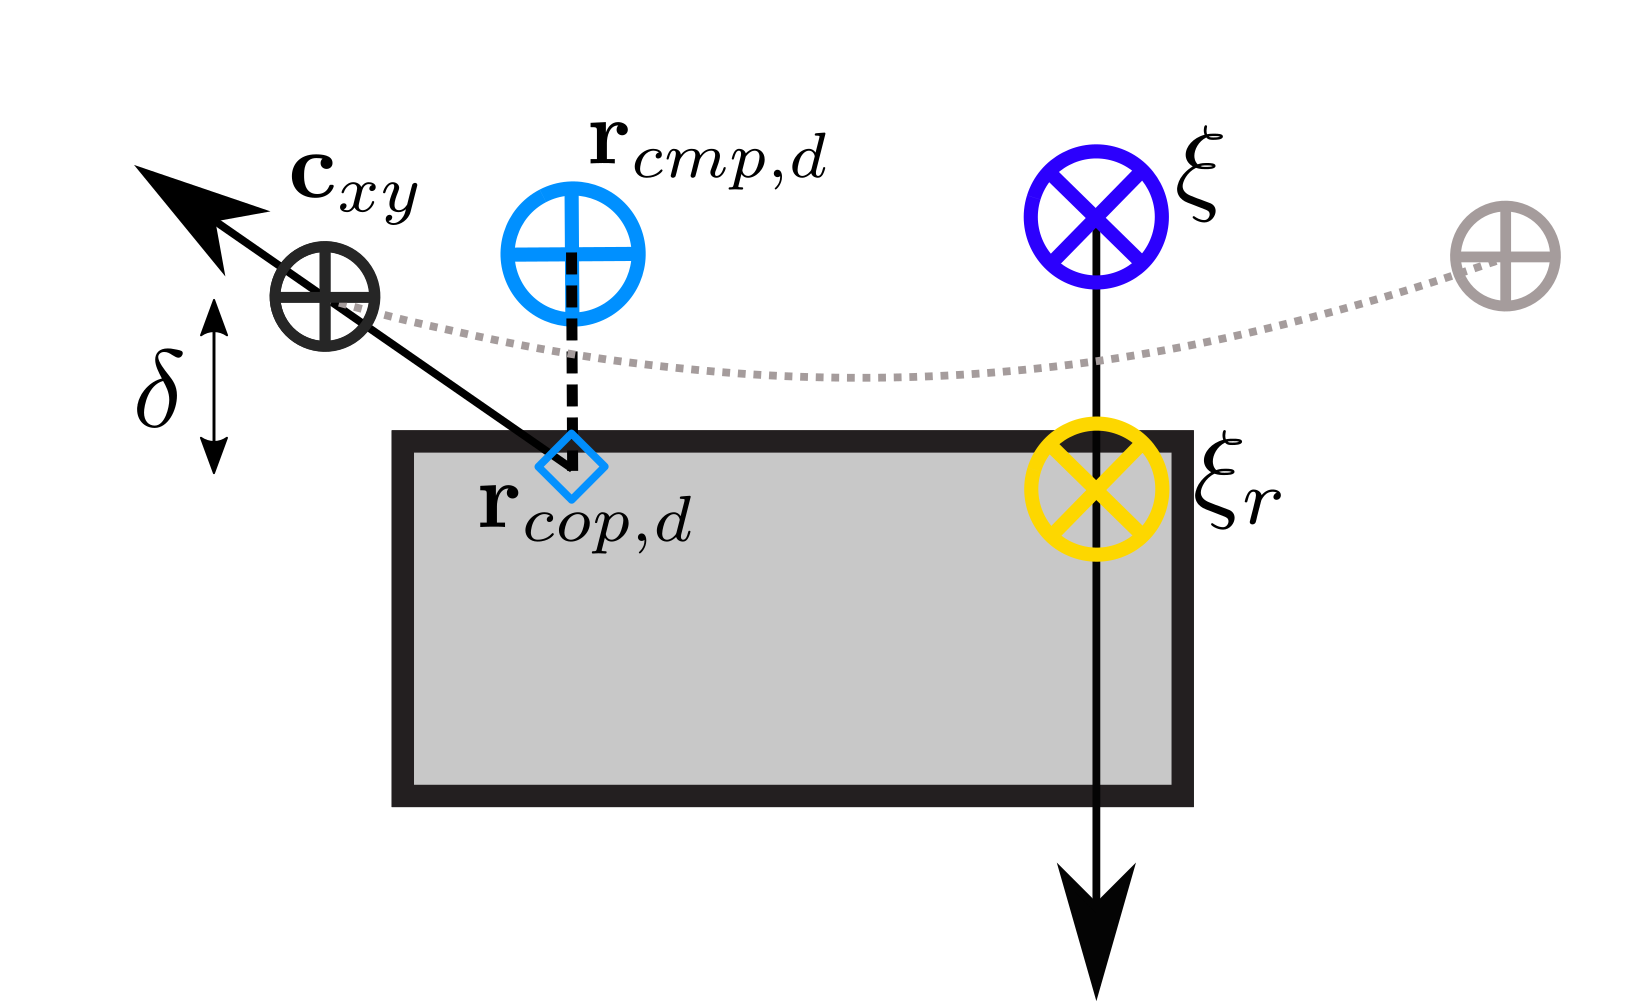
\includegraphics[width=.7\linewidth]{STYLESTUFF/ICPplanStartSSPhiVizRightError.png}
    \caption{}
     \label{fig:phi}
  \end{subfigure}
  \caption{Visualization of $\delta$ and $\phi$ for different error directions. (a) The action `positive alignment' is used. (b) `Prepare' is used. (c) `Positive alignment' is used. (d) `Default' is used.}
  \label{fig:phi}
\end{figure}

For the maximum height constraint $\zmax$, the same parameters as for the standing tests is used in the first half of \ac{SS}. In the second half, the maximum height constraint is linearly interpolated between the maximum height constraint for standing and a maximum height constraint at the end of \ac{SS}.  For the minimum height constraint $\zmin$, a constant value is considered. The height constraints are visually explained in \figref{fig:heightconstraints}.
\begin{figure}
\centering
  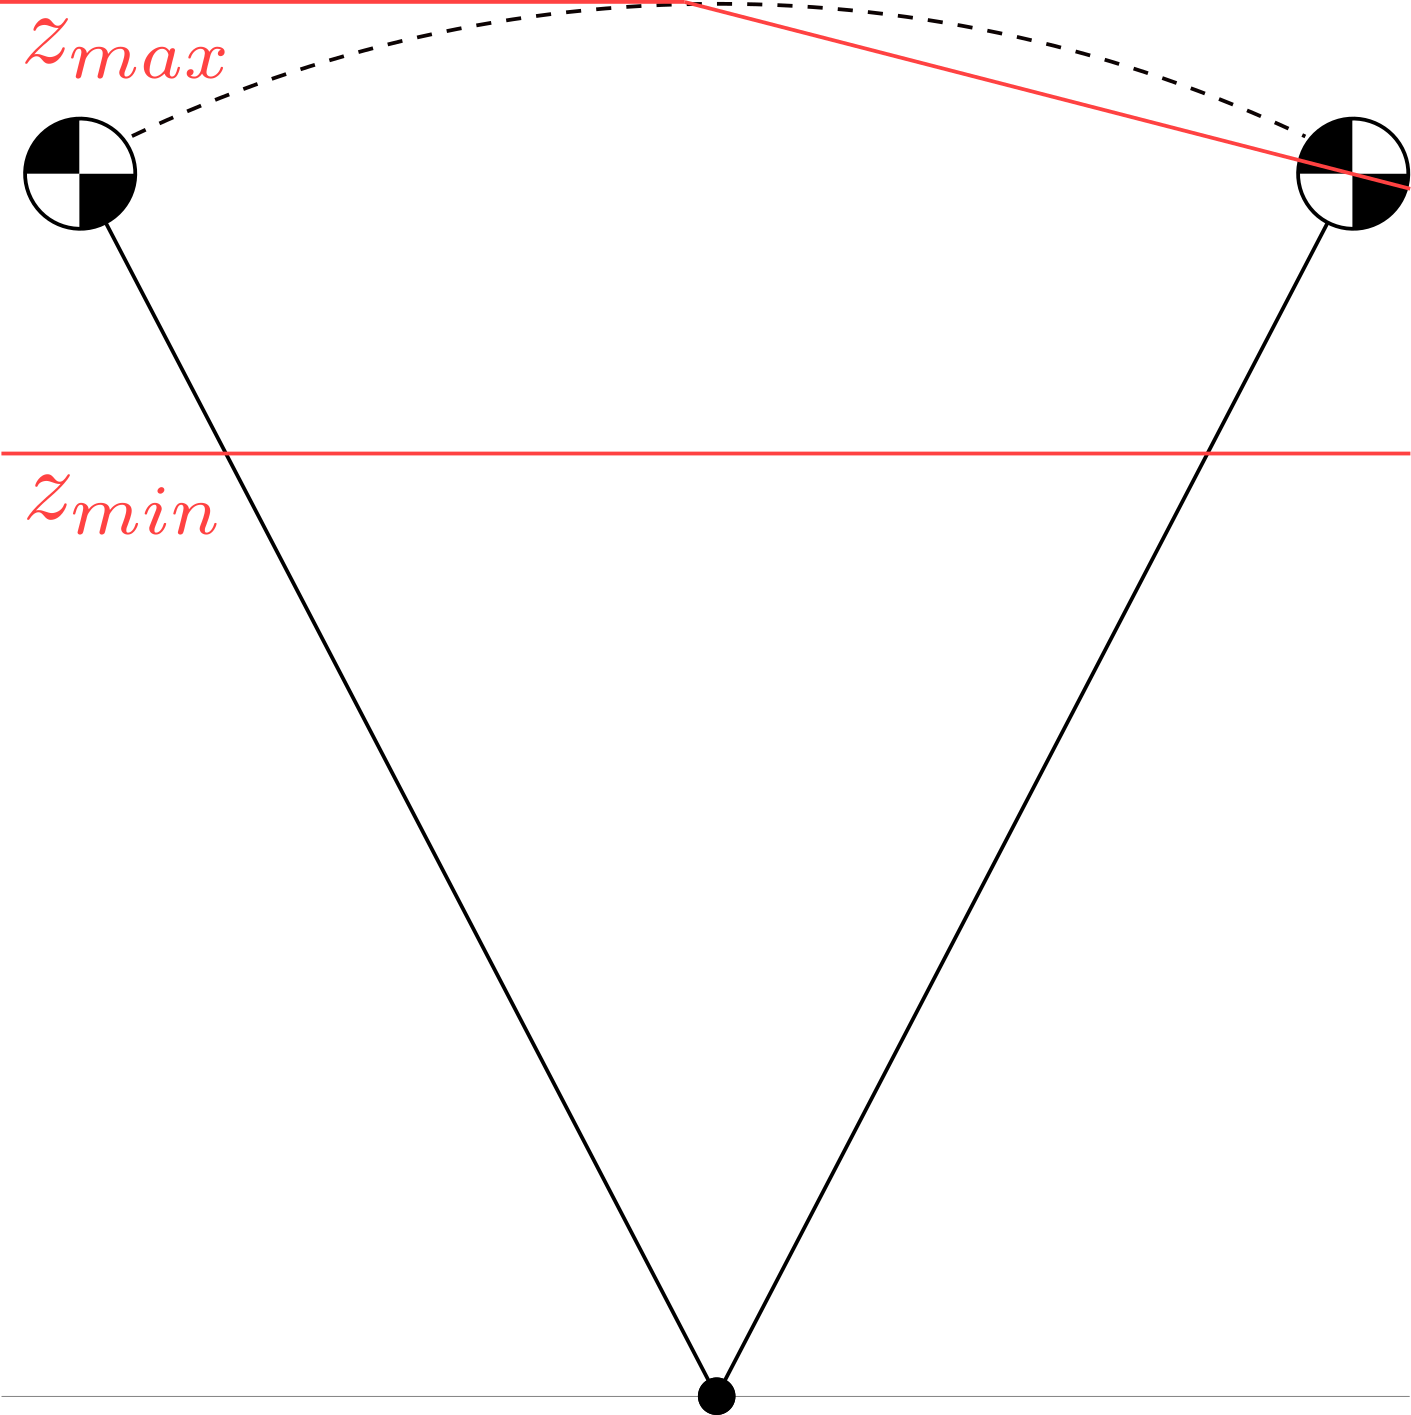
\includegraphics[width=.4\linewidth]{STYLESTUFF/heightconstraints.png}
   \caption{Height constraints through \acf{SS}}
    \label{fig:heightconstraints}
\end{figure} 
\paragraph{The positive alignment action} introduces the bang-bang control law of the previous chapter, using the $\zmax$ as explained above. After the second `bang', the height is not controlled to the maximum height $\zmax$, but is given a feedforward downward acceleration computed with a circle as follows. Consider the distance from the ankle of the robot to the sagittal \ac{CoM} position $x_{ankle}$ and the maximum leg length $l_{max}$. The horizontal position relates to the vertical position as:
\begin{equation}
z^2 = l_{max}^2-x_{ankle}^2.
\end{equation}
The vertical velocity resulting from this function reads as:
\begin{equation}
 \dot{z} = -\frac{x_{ankle}\dot{x}}{\sqrt{l_{max}^2-x_{ankle}^2}}.
\end{equation}
The resulting vertical acceleration reads as:
\begin{equation}
\ddot{z} = \frac{\sqrt{l_{max}^2-x_{ankle}^2}(-\dot{x}^2-x_{ankle}\ddot{x}) - \frac{x_{ankle}^2\dot{x}^2}{\sqrt{l_{max}^2-x_{ankle}^2}}}{ l_{max}^2-x_{ankle}^2}.
\end{equation}
Assuming the sagittal acceleration $\ddot{x}$ is zero, the desired height acceleration is computed as:
\begin{equation}
 \ddzd = -\frac{\dot{x}^2}{\sqrt{ l_{max}^2-x_{ankle}^2}} - \frac{x_{ankle}^2\dot{x}^2}{(l_{max}^2-x_{ankle}^2)^{1\frac{1}{2}}}
\end{equation}
\paragraph{The prepare action} uses the time it takes to accelerate from the minimum height constraint to the maximum height constraint. This time uses the kinetic and potential energy:
\begin{equation}
	\zmin + \frac{1}{2}\ddzc t_{\zmin \rightarrow \zmax}^2 + \frac{1}{2}\frac{(\ddzc t_{\zmin \rightarrow \zmax})^2}{\ddzalpha \ddzc} = \zmax,
\end{equation}
where $t_{\zmin \rightarrow \zmax}$ is the time from the minimum height constraint to the maximum, considering a zero initial vertical velocity.
This solution for the time reads as:
\begin{equation}
 t_{\zmin \rightarrow \zmax}= \sqrt{\frac{2(\zmax - \zmin)}{\ddzc + \frac{\ddzc}{\ddzalpha} }}.
\end{equation}

This time is used to determine the moment when the first `bang' should be activated. The known remaining time in \ac{SS} $t_{r}$ is shortened by $ t_{\zmin \rightarrow \zmax}$:
\begin{equation}
	t_{z \rightarrow \zmin} =t_{r} - t_{\zmin \rightarrow \zmax},
\end{equation}
where $t_{z \rightarrow \zmin} $ is the time available to move from the current height $z$ to the minimum height $\zmin$. Using this time, at every control tick the desired acceleration $\ddzd$ is computed by using the equation:
\begin{align}
	z + \dot{z}t_{z \rightarrow \zmin} + \frac{1}{2}\ddzd t_{z \rightarrow \zmin}^2 - \frac{1}{2}\frac{(\ddzd t_{z \rightarrow \zmin} + \dot{z})^2}{\ddzalpha \ddzc} &= \zmin, \\
	\underbrace{-\frac{1}{2}\frac{t_{z \rightarrow \zmin}^2}{\ddzalpha \ddzc}}_a \ddzd^2 + \underbrace{(\frac{1}{2}t_{z \rightarrow \zmin}^2-\frac{t_{z \rightarrow \zmin}}{\ddzalpha \ddzc} \dot{z})}_b \ddzd + \underbrace{z -\zmin +\dot{z}t_{z \rightarrow \zmin} -\frac{1}{2}\frac{\dot{z}^2}{\ddzalpha \ddzd}}_c&=0,
\end{align}
which has the solution:
\begin{equation}
 	\ddzd = \frac{-b + \sqrt{b^2-4ac}}{2a}.
\end{equation}
This value for $\ddzd$ is used until $t_{z \rightarrow \zmin}<0$, after which the positive `bang' is activated. 

% Results
\section{Results}
The following results are obtained by approximating the effects of $\phi$ and $\delta$ by choosing a phase depending on the direction of the \ac{ICP} error with respect to the sagittal direction.

\begin{figure}
     \centering
    \begin{subfigure}[t]{0.49\textwidth}
     \centering
        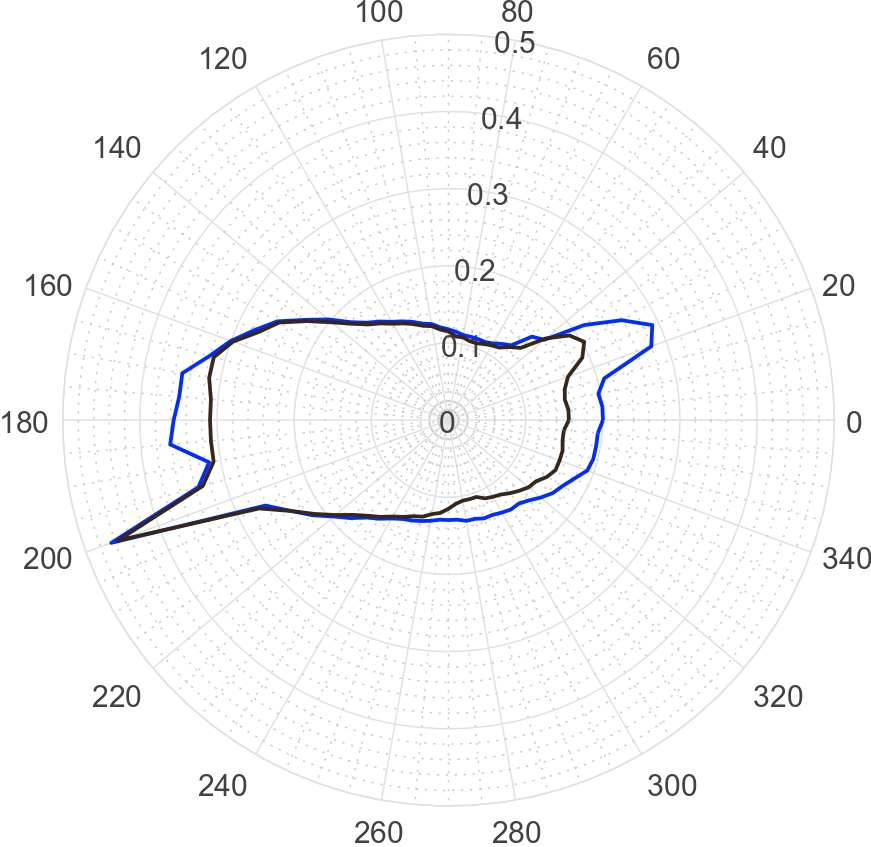
\includegraphics[width=0.8\linewidth]{STYLESTUFF/round00.png}
        \caption{caption of first image}
    \end{subfigure}
    \begin{subfigure}[t]{0.49\textwidth}
     \centering
       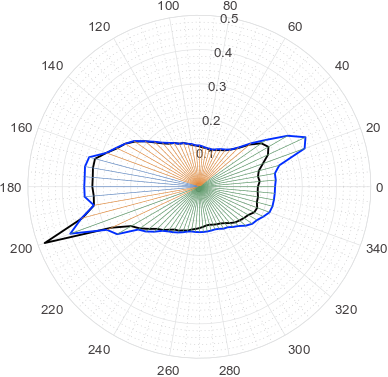
\includegraphics[width=0.8\linewidth]{STYLESTUFF/round01.png}
        \caption{caption of second image}
    \end{subfigure}
    \par\bigskip
   \begin{subfigure}[t]{0.49\textwidth}
    \centering
        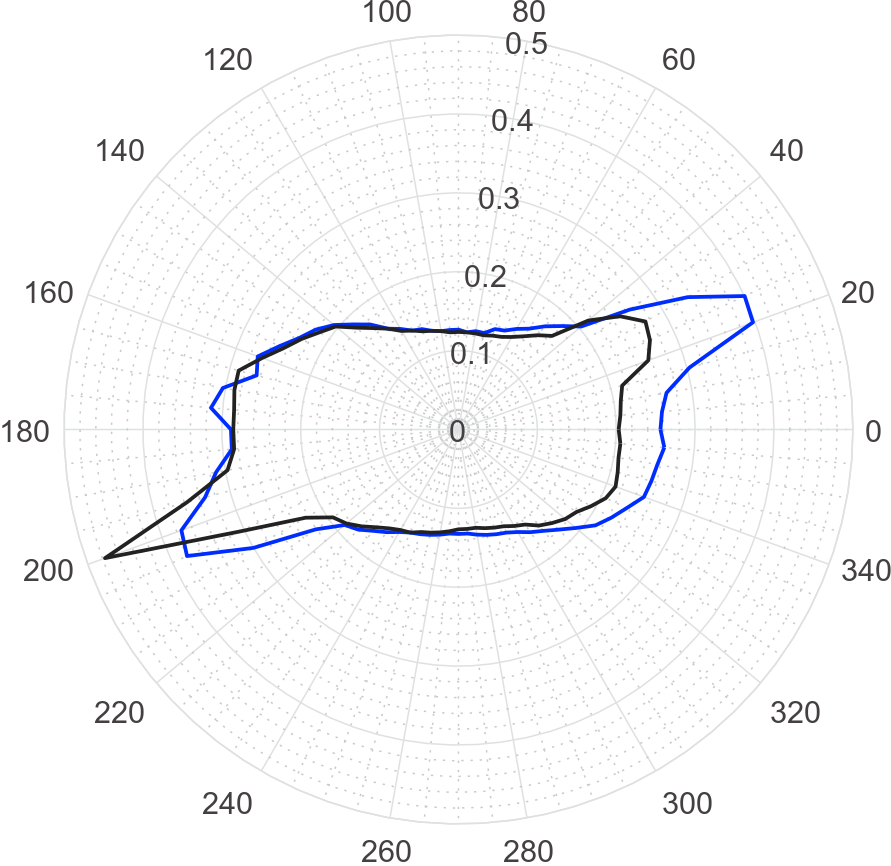
\includegraphics[width=0.8\linewidth]{STYLESTUFF/round02.png}
    \caption{caption of last image} 
    \end{subfigure}
    \begin{subfigure}[t]{0.49\textwidth}
     \centering
        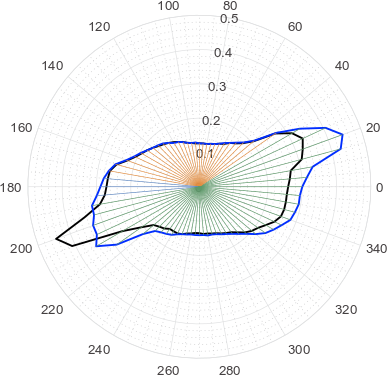
\includegraphics[width=0.8\linewidth]{STYLESTUFF/round03.png}
    \caption{caption of last image} 
    \end{subfigure}
     \par\bigskip
    \begin{subfigure}[t]{0.49\textwidth}
     \centering
        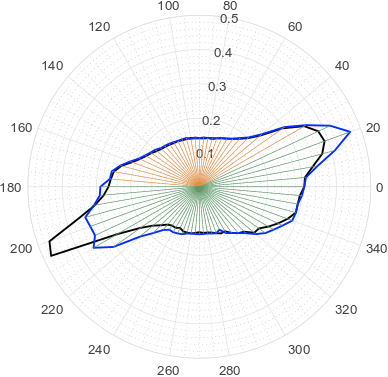
\includegraphics[width=0.8\linewidth]{STYLESTUFF/round04.png}
    \caption{caption of last image} 
    \end{subfigure}
    \begin{subfigure}[t]{0.49\textwidth}
     \centering
        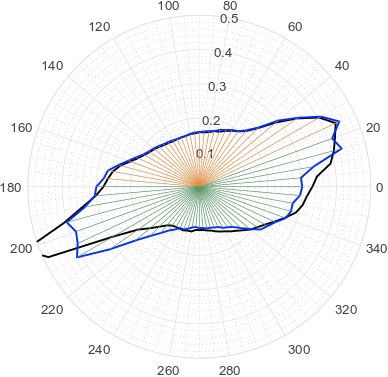
\includegraphics[width=0.8\linewidth]{STYLESTUFF/round05.png}
    \caption{caption of last image} 
    \end{subfigure}
    \caption{caption of main figure}
\end{figure}

\begin{figure}
     \centering
    \begin{subfigure}[t]{0.49\textwidth}
     \centering
        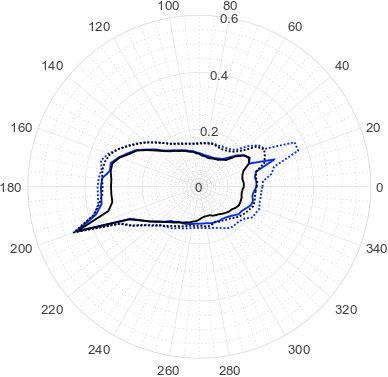
\includegraphics[width=0.8\linewidth]{STYLESTUFF/round00Ang.png}
        \caption{caption of first image}
    \end{subfigure}
    \begin{subfigure}[t]{0.49\textwidth}
     \centering
       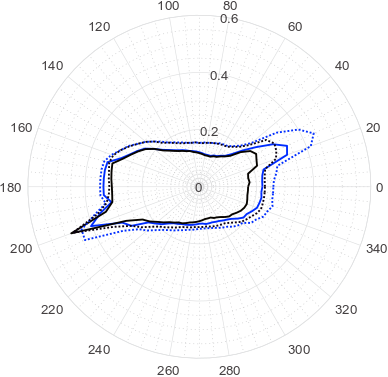
\includegraphics[width=0.8\linewidth]{STYLESTUFF/round01Ang.png}
        \caption{caption of second image}
    \end{subfigure}
    \par\bigskip
   \begin{subfigure}[t]{0.49\textwidth}
    \centering
        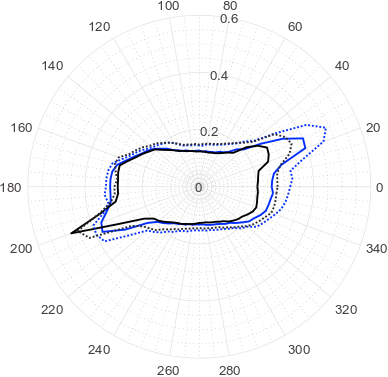
\includegraphics[width=0.8\linewidth]{STYLESTUFF/round02Ang.png}
    \caption{caption of last image} 
    \end{subfigure}
    \begin{subfigure}[t]{0.49\textwidth}
     \centering
        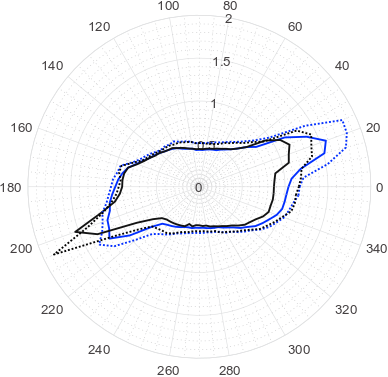
\includegraphics[width=0.8\linewidth]{STYLESTUFF/round03Ang.png}
    \caption{caption of last image} 
    \end{subfigure}
    \par\bigskip
    \begin{subfigure}[t]{0.49\textwidth}
     \centering
        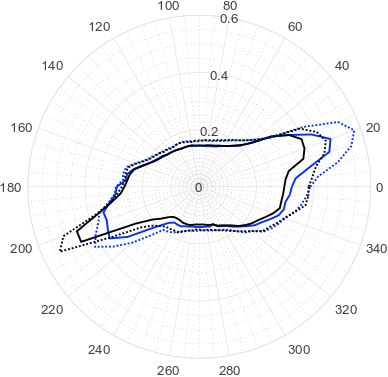
\includegraphics[width=0.8\linewidth]{STYLESTUFF/round04Ang.png}
    \caption{caption of last image} 
    \end{subfigure}
    \begin{subfigure}[t]{0.49\textwidth}
     \centering
        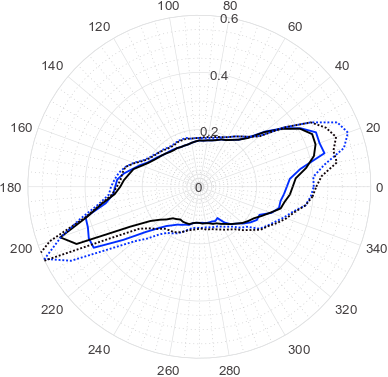
\includegraphics[width=0.8\linewidth]{STYLESTUFF/round05Ang.png}
    \caption{caption of last image} 
    \end{subfigure}
    \caption{caption of main figure}
\end{figure}
% Discussion
\section{Discussion}
